\documentclass[12pt]{article}

\usepackage{amsmath, graphicx}
\usepackage[margin=1in]{geometry}
\usepackage[font=footnotesize]{caption}
\usepackage[backend=bibtex]{biblatex}
\addbibresource{cs221proj.bib}

\DeclareMathOperator*{\argmin}{arg\,min}
\DeclareMathOperator*{\argmax}{arg\,max}


\begin{document}
\nocite{*}

\title{Super Mario Bros with Deep Reinforcement Learning}

\author{
  Matthew Chen\\
  \small \vspace{-2mm} Department of Computer Science\\
  \small \vspace{-2mm} Stanford University\\
  \small mcc17@stanford.edu
  \and
  Isabel Bush\\
  \small \vspace{-2mm} Department of Computer Science\\
  \small \vspace{-2mm} Stanford University\\
  \small ibush@stanford.edu
}
\date{}
\maketitle

\begin{abstract}
We implement a several reinforcement learning models to learn the optimal actions for a variant of the classic Super Mario Bros game. The game is challenging from an AI standpoint as the environment is stochastic with randomly generated levels, and the state space is large. Our algorithms use Q-learning with differing Q-function approximations. We test the effectiveness of the various approximations relative to their performance and runtime.

\end{abstract}

\section{Related Work}

A Super Mario Bros competition started in 2009 as a way to benchmark AI algorithms on the task of creating an effective controller for the game \cite{togelius20102009}. In the first iteration, the best performing agents were ones based on open-loop path planning algorithms such A*. The most successful of these algorithms built an extensive internal model of the game to find optimal paths to the end goal. All other heuristic and learning algorithms were outperformed by a baseline Forward Jumping Agent. The best submissions that involved some form of learning for the follow-up competition were based off of a combination of search and evolutionary algorithms \cite{karakovskiy2012mario}.

Outside of the official competition there have been several attempts at using reinforcement for the simulation, such as Q-learning in \cite{liao2012cs229}. However, this implementation involves hand crafted features and uses a simple lookup as the Q-function approximation. To create a controller that can translate the raw input from the game to optimal actions, we draw inspiration from recent deep learning approaches applied in \cite{mnih2013playing}. In this study, researchers applied a convolutional neural network to map raw pixel values to actions for several Atari games and were able achieve super-human performance on several of the games they tested. In this paper we experiment with this approach to determine if a similar neural network can achieve similar levels of performance in the Mario game, which appears to be a more complex learning task.

\section{Models}

\begin{figure}[h]
\centering
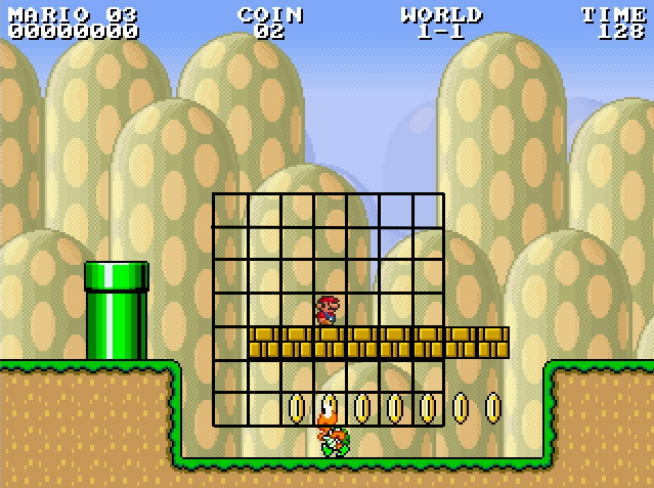
\includegraphics[scale=0.5]{imgs/mario_grid}
\caption{A component of the game state is a small grid centered around Mario indicating objects nearby. In the actual simulation, the grid is 22 x 22 cells, where each cell is the size of a single block \cite{karakovskiy2012mario}.}
\label{mario_grid}
\end{figure}

We choose the Q-Learning algorithm as our approach to this problem as it enables us to learn a controller without creating a model for the game or having a fixed reward function. Our approach experiments with different Q-function approximations such as identity, linear, and neural network. Additionally we employ an epsilon greedy strategy to ensure adequate exploration of the state space by taking a random action with probability 1 - $\epsilon$. The update rule and optimal action choice are as follows, where R(s') is the reward for ending in state s' after taking action a at state s.

\begin{align*}
Q(s,a) &\leftarrow Q(s,a) + \alpha (R(s') + \gamma \max_{a' \in A} Q(s',a') - Q(s,a))\\
a^* &= \argmax_{a \in A} Q(s,a)
\end{align*}

Our state is defined as a vector of all observed attributes of the game. This can be divided into two components. In the first component are meta data features which include distance to the finish, time left, and Mario state (small, large, fireball power). These features describe the progression of the game. The second component is a 22 x 22 grid which is provided by the simulator at each time step, as shown in Figure \ref{mario_grid}. The grid can be thought of as a low detail/resolution view of the game. The entire grid is centered around Mario and each cell corresponds to objects in that relative position to Mario (blocks, mushrooms, monsters, gap, etc). We flatten this grid to get the underlying features.

Actions correspond to combinations of the original buttons which could be pressed for the player to interact with the game. The game uses a six element vector corresponding to the set of six buttons which can be toggled on and off during a given time-step (directional move, jump, and fireball). Since combinations of buttons are possible, we have defined our set of possible actions as all binary combinations of the six buttons leading to $2^6 = 64$ distinct actions.

The reward at each time-step is calculated as the change in fitness score over that time-step due to the action taken at the previous state. The fitness score takes into account distance passed and coins collected.

\subsection{Identity Function}

Our first learning agent maps the full state representation vector to the best action to take from that state. Since the state space is very large (the state vector has length $733$, which yields upwards of $2^{733}$ distinct states) and many states are unlikely to be seen (creating a sparse feature vector), we stored the state-action mapping in a hashmap to allow for quick access and efficient space usage. This was the strategy deployed by \cite{liao2012cs229}, except their representation of state required high-level hand-crafted features while our representation uses low-level game features. Below we specify the Q function and corresponding basis function which transforms a state action pair to the given state vector representation.

\begin{align*}
Q(s,a) &= Lookup(\beta(s,a))\\
\beta(s,a)_{i*j} &= 1\{ S_i = s \} * 1\{ A_j = a \}
\end{align*}

\subsection{Linear Approximation}


Our linear agent uses the same low-level game features, but fits a linear model to estimate the value function. This model approximates the Q-function by taking a dot product between a vector of learned weights and the input features. The feature vector consists of indicator values for each element of the state vector and every possible action. This yields a feature vector of length $|stateVector| * |Actions| = 733 * 64 = 46,912$. While still large, this is much less than the identity feature vector and can easily fit in memory. And more importantly, this allows the agent to generalize to unseen states and learn more quickly.

\begin{align*}
Q(s,a) &= \theta^T \beta(s,a)\\
\beta(s,a)_{i*j} &= 1\{ S_i = s \} * 1\{ A_j = a \}
\end{align*}

\subsection{Neural Network}

Our neural network implementation has even fewer input features than the linear agent. Since state/action interactions can be exposed by the network, the input feature vector can be simplified to the state vector and an indicator for the action chosen. The features are fed through two fully-connected layers, with associated rectified linear layers, to the final fully-connected output layer which provides an estimate for the Q-function.

\begin{align*}
Q(s,a) &= ForwardPass(\theta, \beta(s, a))\\
\beta(s,a)_{i} &= 1 \{ S_i = s \}\\
\beta(s,a)_{|S| + j} &= 1 \{ A_j = a \}
\end{align*}

Additionally, we experiment with using a playback memory as defined in \cite{mnih2013playing}. We store the previous N observations from the game. We then sample from these observations during a single update to perform mini-batch gradient descent. This method is used to help mitigate the problem of correlated features from time windows and aid in the convergence of the weights.

\section{Results}

\subsection{Method Comparison}

\begin{figure}
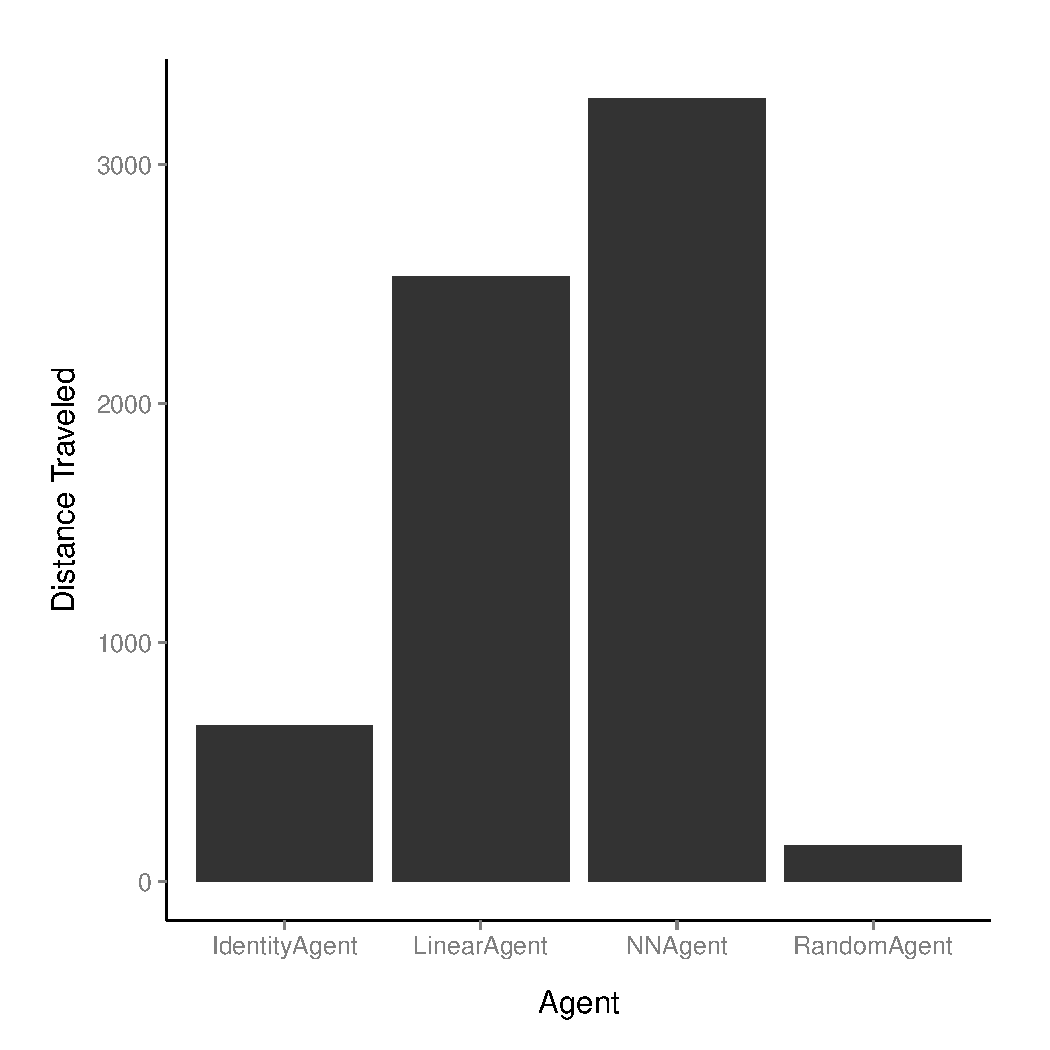
\includegraphics[scale=0.5]{imgs/dist_bar.pdf}
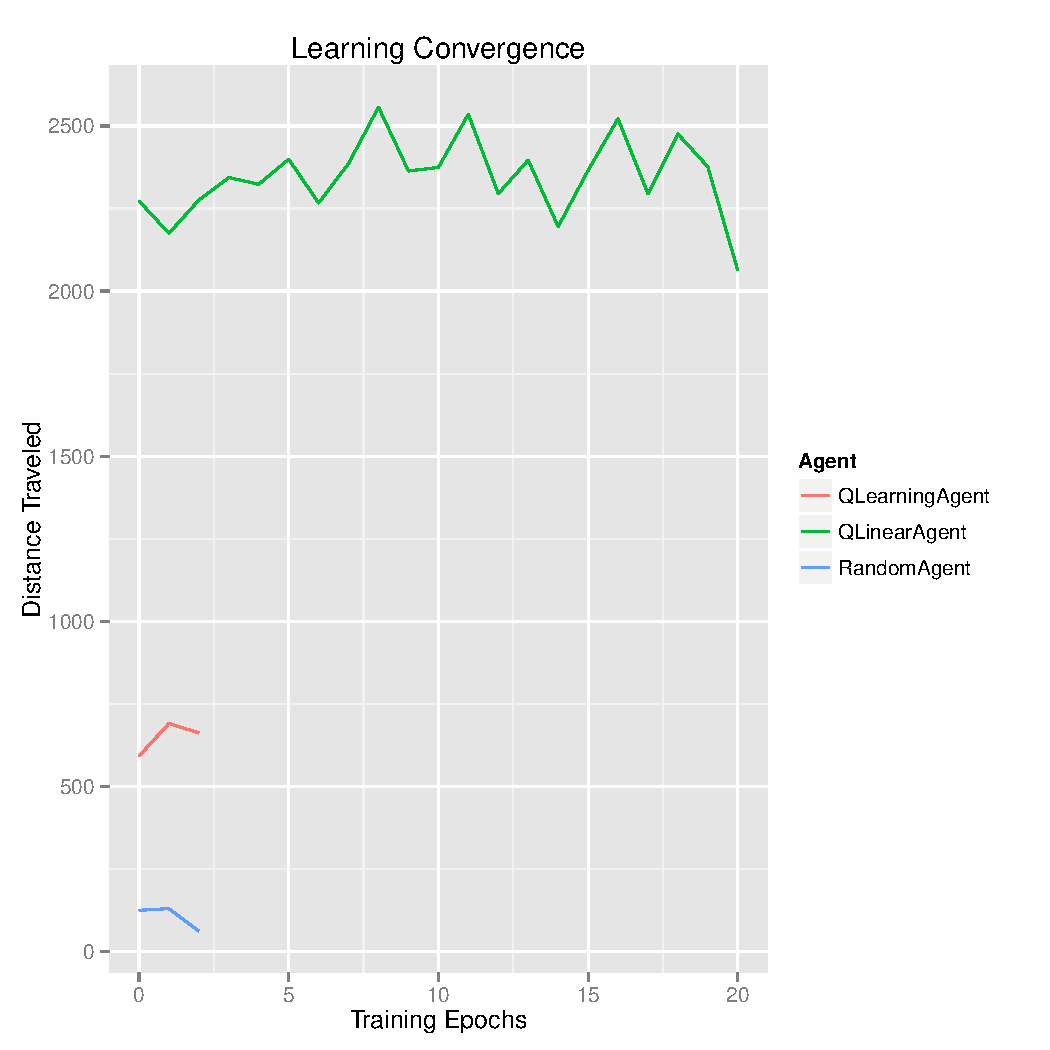
\includegraphics[scale=0.5]{imgs/dist_line.pdf}
\caption{Learning statistics showing comparison between different agents by mean progress before end of game}
\label{agent_comp}
\end{figure}

We implemented initial versions of the Identity and Linear Approximation Agents, as well as a baseline random agent that chooses a random action at each step. Preliminary results show that both models are able to learn some of the game's goals and outperform the random agent by a large margin as shown in Figure \ref{agent_comp}.

The Identity Agent was able to run for about 200 trials before running out of memory (where each trial is a full game and consists of about 1000 time-steps). At the start of learning, Mario jumps around aimlessly performing random actions. By the end of the 200 trials, the agent has learned to move forward from some states and thus makes progress. However, since there is no generalization, the agent still performs random actions from some states and the game usually ends due to time-out. 

The distance travelled over the trials for the agents can be seen in the Learning Convergence graph in Figure \ref{agent_comp}. While there is much variability, the trend is positive for the Identity Agent. Over the last 50 trials, the Identity Agent travelled an average distance of 710 with an average fitness score of 1,561. This is significantly better than the baseline random agent, which travels an average distance of 127 with an average fitness score of 257.

Due to generalization of state features, the Linear Agent learns much faster than the Identity Agent, as can be seen by the higher distance travelled even during the first few training epochs. The rate is faster despite a much lower learning rate (step-size), which was needed to keep the weights from diverging. The Linear Agent is able to progress farther on average than the Identity Agent (generalizing the desire to move forward to many different states) and thus usually completes the level or dies from a monster rather than hitting the timeout. The Linear Agent travels an average distance of 2,360 with an average fitness score of 5,140, far outperforming both the random agent and Identity Agent.

\subsection{Runtime Analysis}

\subsection{NN Parameter Tuning}

\section{Discussion}

We start our Q Learning agent with the identity agent which attempts to map low level features to a value. While this is a simple model, it has a few shortcomings. First, since this simple Q learning model maps directly from states to actions, no generalization may be made to unseen states. The best action to take from each state must be learned independently, and the agent will choose a random action for any new state (even if very similar to a past state). This makes learning slow and inefficient. Second, an implementation shortcoming of this model is that the large feature vector consisting of all possible states can overflow memory. This limits the number of learning trials that may be run as the memory-usage grows with each new state.

Next our linear agent attempted to solve these issues by having a linear function approximation for the Q value. This method allowed us to store information about states in a fixed size $\theta$ vector. It also allowed for generalization unseen states were given a score with some basis in experience. The method linear agent performed very well relative to our baseline method and the identity agent for these reasons. The issue for the linear agent is the linear assumption in the function approximation is likely too constraining to get a good estimate as to the true Q value function. This is due to the fact that the features, such as the grid input, are not independent of one another.

Our Q agent with a neural network function approximation aimed to address some of the limitations of the linear function approximation. The use of several hidden layers with rectified linear unit non-linearities allows us to approximate more complex functions. Additionally, in order to help the convergence of the weights, we implemented replay memory to store previous observations and randomly sample a subset for each update. This lead to a agent that performed better than our linear agent. However this performance came at a cost in terms of runtime as it took significantly longer to compute each move relative to our other approaches.





\printbibliography

\end{document}